\documentclass{package/notes}
\usepackage[english]{babel}
\usepackage{amssymb,amsmath,amsfonts}  %%% for maths
%%%%%%%%%%%%%%%%%%%%%%%%%%%%%%%%%%%%%
\usepackage{package/color-env}
\usepackage{lipsum}
\usepackage{longtable,booktabs,calc}

\newcommand{\Z}{\mathbb{Z}}
\newcommand{\R}{\mathbb{R}}
\newcommand{\N}{\mathbb{N}}
\newcommand{\C}{\mathbb{C}}
\newcommand{\Q}{\mathbb{Q}}
\newcommand{\lcm}{\text{ lcm}}
\renewcommand\qedsymbol{$\blacksquare$}
%%%%%%%%%%%%%%%%%%%%%%%%%%%%%%%%%%%%%

\begin{document}

	\begin{titlepage} % Suppresses headers and footers on the title page
		
		\centering % Centre everything on the title page
		
		\scshape % Use small caps for all text on the title page
		
		\vspace*{\baselineskip} % White space at the top of the page
		
		%------------------------------------------------
		%	Title
		%------------------------------------------------
		
		\rule{\textwidth}{1.6pt}\vspace*{-\baselineskip}\vspace*{2pt} % Thick horizontal rule
		\rule{\textwidth}{0.4pt} % Thin horizontal rule
		
		\vspace{0.75\baselineskip} % Whitespace above the title
		
		{\huge MATH231 Discrete Structures Notes\\} % Title
		
		\vspace{0.75\baselineskip} % Whitespace below the title
		
		\rule{\textwidth}{0.4pt}\vspace*{-\baselineskip}\vspace{3.2pt} % Thin horizontal rule
		\rule{\textwidth}{1.6pt} % Thick horizontal rule
		
		\vspace{2\baselineskip} % Whitespace after the title block
		
		%------------------------------------------------
		%	Subtitle
		%------------------------------------------------
		
		
		
		\vspace*{3\baselineskip} % Whitespace under the subtitle
		
		
		
		\vspace{0.5\baselineskip} 
		
		
		
		\vspace{0.5\baselineskip} 
		
		
		
		\vfill 
		
		%------------------------------------------------
		% Author
		%------------------------------------------------
		
		
		\vspace{0.3\baselineskip} 
		
		
		{\large Edited by\\  Trevor Bushnell} 
		
	\end{titlepage}
	\tableofcontents
%\newpage
\chapter*{Introduction}

This document aims to highlight the important content of the MATH231 course in traditional notes format. These notes are completely open-source, which means anyone is allowed to use these notes for their own personal benefit without having to seek permission from myself. \newline

Due to the open-source nature of these notes, anyone is allowed to contribute to improving these notes as they see fit. Since I am using \LaTeX to write these notes and I am using GitHub to distribute these notes easily, you must request all changes through the repository website on GitHub, which you can find \textbf{here}. If you are interested in contributing to these notes, then there are a few ways that you can do so:\newline

\begin{enumerate}
	\item \textbf{Open and submit an issue on my GitHub repository:} I write all my notes in \LaTeX, which is a typesetting language that is really helpful when it comes to typing and rendering math equations quickly and easily. If you do not know how to write \LaTeX code but are still interested in making a change to the notes, you can open an issue by going to the MathNotes repo on GitHub, and clicking on the button labeled "New Issue." From there, you can type out the change that you wish to see in the notes. It would be helpful if you would indicate what course you would like to see changed so that I can understand what you are referring to. I will then update the code to include your issue so that you don't have to worry about writing the code yourself.
	\item \textbf{Create and submit a pull request:} If you know how to write LaTeX code and you understand how GitHub works, you can submit a pull request where you can write the code that you want to change yourself. I will then review the code and either submit the code to be incorporated into the notes OR provide some comments on your code if I wish for something to be different. 
\end{enumerate}

Thank you so much for using these notes. I hope that the information is provided in such a way that it can help you when reviewing content for you AP test/class exam and just in general when it comes to learning the content for the course. Happy studying!


\chapter{Logic and Proofs}



\chapter{Basic Structures}



\chapter{Number Theory and Cryptography}
\section{Integers and Divisibility}

While $\Z$ is not closed under division (an integer divided by an integer is not always an integer), we can still come up with definitions for dividing integers. 

\begin{definition}{def3.1}
    If $a,b\in\Z$ and $a\ne 0$, then $a$ \textbf{divides} $b$ ($a|b$) if there exists an integer $k$ such that $ak = b$. In this case, $a$ is a \textbf{factor/divisor} of $b$, and $b$ is a \textbf{multiple} of $a$. If $a$ does not divide $b$, then the notation is $a \nmid b$.
\end{definition}

\begin{itemize}
    \item $2|10$ because $2(5)=10$ where $k=5$
    \item $4 \nmid 10$ because $\frac{10}{4} = 2.5$ which is not an integer
    \item $-6|42$ because $-6(-7)=42$ where $k=-7$
\end{itemize}


\begin{theorem}[The Divisibility Theorem]{theorem3.1:label}
    Let $a,b,c \in \Z$ where $a \ne 0$. Then the following statements are true:

    \begin{itemize}
        \item $a|a$
        \item $a|0$
        \item If $a|b$ and $a|c$, then $a|(b+c)$
        \item If $a|b$, then $a|bc$ for all integers $c$
        \item If $a|b$ and $b|c$, then $a|c$
    \end{itemize}
\end{theorem}

\begin{corollary}[Corollary to the Divisibility Theorem]{cor3.1:label}
    Let $a,b,c\in \Z$ where $a\ne 0$. If $a|b$ and $b|c$, then $a | (mb + nc)$ for all integers $m$ and $n$.
\end{corollary}

\subsection{The Division Algorithm}

\begin{itemize}
    \item Let $a \in \Z$ and $d \in \Z^+$
    \item There are unique integers $q$ and $r$ such that $a = dq + r$ where $0 \le r < d$
    \item $a$ is the \textit{dividend}
    \item $d$ is the \textit{divisor}
    \item $q$ is the \textit{quotient}
    \item $r$ is the remainder 
\end{itemize}

\textbf{THE $\div$ OPERATION:} $a \div b$ means divide $b$ by $a$ and leave off the remainder. 

\begin{itemize}
    \item EX: $4 \div 10 = 2$ because $\frac{10}{4} = 2.5$ and we just care about the whole number part of the answer and disregard the remainder.
\end{itemize}

\textbf{THE $\mod$ OPERATOR:} $a \mod b$ means divide $b$ by $a$ and leave JUST the remainder.

\begin{itemize}
    \item EX: $4 \mod 10 = 2$ because $\frac{10}{4} = 2\text{ R}2$ and we just care about the remainder part of the answer (2)
\end{itemize}

\begin{problem}
    If 100 is divided by 23, write as $a=dq+r$ and find the quotient and remainder.

    $$
    \begin{aligned}
        100 &= 23q + r\\
        100 &= 23 \cdot 4 + 8\\
        100 \div 23 = 4\\
        100 \mod 23 = 8
    \end{aligned}
    $$
\end{problem}

\begin{problem}
    If -100 is divided by 23, write as $a=dq+r$ and find the quotient and remainder.

    $$
    \begin{aligned}
        -100 &= 23q + r
        -100 &= 23(-4) + (-8)\\
        \text{remainder can't be negative so we add another factor of 23 to make the remanider positive}
        -100 &= 23(-5) + 15\\
        -100 \div 23 = -5\\
        -100 \mod 23 = 15
    \end{aligned}
    $$
\end{problem}


\subsection{Introduction to Congruence}

\begin{definition}[Modular Congruence]{def3.2:label}
    Let $a$ and $b$ be integers and let $n$ be a positive integer. Then $a$ and $b$ are \textbf{congruent modulo $n$} if $n|(a-b)$. If $a$ and $b$ are congruent moduo $n$, we then write that $a \equiv b (\mod n)$
\end{definition}

\textbf{NOTE:} $a$ and $b$ are congruent modulo $n$ when the have the same remainder when divided by $n$. This means that if $a$ and $b$ are congruent modulo $n$, then $a \mod n = b \mod n$.

\begin{itemize}
    \item $12 \equiv 2 \mod 5$ because $12 \mod 5 = 2 = 2 \mod 5$
    \item $-7 \not\equiv 2 \mod 5$ because $-7 \mod 5 = 3 \ne 2 \mod 5$
\end{itemize}

\textbf{NOTE:} $\{5k + 2 | k \in \Z\}$ is the set of numbers congruent to a modulo $n$



\section{Integer Representations and Algorithms}

\subsection{Integers in Different Bases}

\begin{theorem}[Integers in Differen Bases]{theorem3.2:label}
    Let $b \in \Z$ and $b > 1$. Then if $n \in \Z^+$, it has a unique base-$b$ expansion, expressed uniquely in the form:

    $$
    n = a_kb^k + a_{k-1}b^{k+1} + \cdots + a_1b^1 + a_0
    $$

    Where $k$ is a non-negative integer and $a_0,a_1,a_2,\cdots,a_k$ are all non-negative integers that are less than $b$ and $a_k \ne 0$.
\end{theorem}

\begin{itemize}
    \item We denote what base we are in by using a subscript equivalent to the base: $(a_ka_{k-1}...a_1a_0)_b$
    \item $b = 10$ is \textit{decimal} expansion
    \item $b = 2$ is \textit{binary} expansion
    \item $b=8$ is the \textit{octal} expansion
    \item $b = 16$ is the \textit{hexaedcimal} expansion
\end{itemize}

\begin{problem}
    Convert $(10010111)_2$ to decimal.

    $$
    \begin{aligned}
        (10010111)_2 &= 1 \cdot 2^7 + 0 \cdot 2 ^6 + 0 \cdot 2 ^5 + 1 \cdot 2 ^4 + 0 \cdot 2 ^3 + 1 \cdot 2 ^2 + 1 \cdot 2 ^1 + 1 \cdot 2 ^0\\
        &= 128 + 16 + 4 + 2 + 1\\
        &= 151
    \end{aligned}
    $$
\end{problem}


\begin{problem}
    Convert $(A1F)_{16}$ to decimal.
\end{problem}


\begin{problem}
    Convert $(1036)_8$ to decimal.
\end{problem}


\subsection{Converting From Base-10 to Base-$n$}


To convert a number from base-10 to base-$n$, you repeatedly use the division algorithm in the following way:

$$
\begin{aligned}
    n &= bq_0 + r_0\\
    q_0 &= bq_1 + r_1\\
    q_1 &= bq_2 + r_2\\
    &...\\
    q_{k-1} = bq_k + r_k
\end{aligned}
$$

You stop this process when $q_k$ is equal to 0. Then, the number in base $n$ is the list of all $r_n$ (all the remainders) in reverse order (so from the bottom step remainder to the first step remainder).

\begin{problem}
    Convert $(108)_10$ into the following bases:

    \begin{itemize}
        \item Binary:
        \item Octal:
        \item Hexadecimal:
    \end{itemize}
\end{problem}


\subsection{Converting From Base-$n$ to Base-$m$}

Every three digits in binary correspond to one octal digit. Similarly, every four digits in binary correspond to one hexadecimal digit.\\

On the next page, you can see a chart matching all of the base 10 numbers from 0-16 and what each number's binary, octal, and hexadecimal representations are. You can then use this table to convert any number in base 2,4,8,16 to base 2,4,8,16.\newpage

\begin{longtable}[]{@{}llll@{}}
    \toprule
    Decimal & Binary & Octal & Hexadecimal \\ \addlinespace
    \midrule
    \endhead
    0 & 0 & 0 & 0 \\ \addlinespace
    1 & 1 & 1 & 1 \\ \addlinespace
    2 & 10 & 2 & 2 \\ \addlinespace
    3 & 11 & 3 & 3 \\ \addlinespace
    4 & 100 & 4 & 4 \\ \addlinespace
    5 & 101 & 5 & 5 \\ \addlinespace
    6 & 110 & 6 & 6 \\ \addlinespace
    7 & 111 & 7 & 7 \\ \addlinespace
    8 & 1000 & 10 & 8 \\ \addlinespace
    9 & 1001 & 11 & 9 \\ \addlinespace
    10 & 1010 & 12 & A \\ \addlinespace
    11 & 1011 & 13 & B \\ \addlinespace
    12 & 1100 & 14 & C \\ \addlinespace
    13 & 1101 & 15 & D \\ \addlinespace
    14 & 1110 & 16 & E \\ \addlinespace
    15 & 1111 & 17 & F \\ \addlinespace
    16 & 10000 & 20 & 10 \\ \addlinespace
    \bottomrule
\end{longtable}

\begin{problem}
    Convert $(DB5)_{16}$ into binary and octal.
\end{problem}


\section{Primes and Greatest Common Divsors}

\begin{definition}[Prime Numbers]{def3.3.1:label}
    An integer $p$ greater than 1 is \textbf{prime} if the only positive factors of $p$ are 1 and $p$.
\end{definition}

\begin{theorem}[The Fundamental Theorem of Arithmetic]{theorem3.3.1:label}
    Every integer greater than 1 can be written uniquely as a prime or as the prodct of two or more primes written in increasing order.
\end{theorem}

\begin{problem}
    Fnid the prime factorizations of the following numbers:

    \begin{itemize}
        \item $36 = 6^2 = (2\cdot 3)^2 = 2^2\cdot 3^2$\\
        \item $84 = 7 \cdot 12 = 7 \cdot 3 \cdot 2 \cdot 2 = 2^2\cdot 3 \cdot 7$
        \item $31 = 31 \cdot 1$
    \end{itemize}
\end{problem}

\begin{proposition}{prop3.3.1:label}
    If $n$ has a prime divisor, then it must have one that is less than or equal to $\sqrt{n}$
\end{proposition}

Listed below is a table with all of the primes that are $\le 100$. Every number that is \textbf{bold} is a prime number.

\begin{longtable}[]{@{}llllllllll@{}}
    \toprule
    1 & \textbf{2} & \textbf{3} & 4 & \textbf{5} & 6 & \textbf{7} & 8 & 9 &
    10 \\ \addlinespace
    \textbf{11} & 12 & \textbf{13} & 14 & 15 & 16 & \textbf{17} & 18 &
    \textbf{19} & 20 \\ \addlinespace
    21 & 22 & \textbf{23} & 24 & 25 & 26 & 27 & 28 & \textbf{29} &
    30 \\ \addlinespace
    \textbf{31} & 32 & 33 & 34 & 35 & 36 & \textbf{37} & 38 & 39 &
    40 \\ \addlinespace
    \textbf{41} & 42 & \textbf{43} & 44 & 45 & 46 & \textbf{47} & 48 & 49 &
    50 \\ \addlinespace
    51 & 52 & \textbf{53} & 54 & 55 & 56 & 57 & 58 & \textbf{59} &
    60 \\ \addlinespace
    \textbf{61} & 62 & 63 & 64 & 65 & 66 & \textbf{67} & 68 & 69 &
    70 \\ \addlinespace
    \textbf{71} & 72 & \textbf{73} & 74 & 75 & 76 & 77 & 78 & \textbf{79} &
    80 \\ \addlinespace
    81 & 82 & \textbf{83} & 84 & 85 & 86 & 87 & 88 & \textbf{89} &
    90 \\ \addlinespace
    91 & 92 & 93 & 94 & 95 & 96 & \textbf{97} & 98 & 99 &
    100 \\ \addlinespace
    \bottomrule
    \end{longtable}


\begin{theorem}{3.3.2:label}
    There are infinietly many primes.
\end{theorem}

\begin{definition}{3.3.2:label}
    Let $a$ and $b$ be integers with $a$ and $b$ not being equal to 0. The largest integer $d$ such that $d|a$ and $d|b$ is called the \textbf{greatest common divisor} of $a$ and $b$. The notation is $\gcd(a,b)$
\end{definition}

\begin{problem}
    Find $\gcd(36,84).$

    $$
    \begin{aligned}
        36 &= 6 \cdot 6 = 2^2 \cdot 3^2\\
        84 &= 7 \cdot 12 = 2^2 cdot 3 \cdot 7\\
        \gcd(36,84) &= 2^2 \cdot 3 = 12
    \end{aligned}
    $$
\end{problem}

\begin{problem}
    Find $\gcd(9,49).$

    $$
    \begin{aligned}
        9 &= 3^2\\
        49 &= 7^2\\
        \gcd(9,49) &= 1
    \end{aligned}
    $$
\end{problem}


\begin{definition}[Relatively Prime]{def3.3.3:label}
    Two integers $a$ and $b$ are \textbf{relatively prime} if $\gcd(a,b) = 1$.
\end{definition}


\begin{definition}{def3.3.4:label}
    The least common multiple of the positive integers $a$ and $b$ is is the smallest positive integer that is divisible by both $a$ and $b$. Notation is $\lcm(a,b)$.
\end{definition}


\chapter{Induction and Reasoning}
\section{Introduction to Work}

\begin{definition}{def4.1:label}
    \textbf{WORK: How much energy it takes to do a certain physical action.}

    $$
    W = \Delta E = \vec F \cdot \vec {\Delta x}
    $$

    $W$ = Work done (SI Units: $\J = \N\m$)\\
    $\Delta E$ = Change in energy\\
    $\vec F$ = the force applied\\
    $\Delta x$ = the displacement over which the object was applied the given force $\vec F$
\end{definition}


\begin{problem}
    A couch is pushed with a force 25 $\N$ over a distance of 5 $\m$. Calculate the work that is applied to the couch. 

    $$
    \begin{aligned}
        W &= F_A \cdot \Delta x\\
        W &= (25 \N)(5 \m)\\
        W &= 100 \J
    \end{aligned}
    $$
\end{problem}


\begin{problem}
    \textbf{SEE ATTACHED FIGURE}

    a) How much energy is expended by the applied force to move the couch 5 $\m$?
    b) How much energy does the frictional force expend to move the couch 5 $\m$?

    To solve part a):
    $$
    \begin{aligned}
        W_A &= F_{Ax} \cdot \Delta x\\
        W_A &= F\cos\theta \cdot \Delta x\\
        W_A &= (50 \N)\cos(25^\circ)(5 \m)\\
        W_A &= 227 \J
    \end{aligned}
    $$

    To solve part b):
    $$
    \begin{aligned}
        W_f &= -F_f \cdot \Delta x\\
        W_f &= -\mu_kF_N \cdot \Delta x\\
        W_f &= -\mu_k(mg + F_A\sin\theta) \cdot \Delta x\\
        W_f &= -(0.15)((20\kg)(9.81\frac{\m}{\s^2}) + (50\N)\sin(25^\circ))
        W_f &= VALUE
    \end{aligned}
    $$
\end{problem}


\section{Energy}

Energy comes in many different forms. The main forms of energy (as well as the proofs to get their respective equations) are listed below:


\begin{definition}[Kinetic Energy]{def4.2:label}
    If an object is moving, the energy that the object expends is equal to the \textbf{kinetic energy}. 

    $$
    KE = \frac{1}{2}mv^2
    $$

    $KE$ = the kinetic energy expended\\
    $m$ = mass of the object\\
    $v$ = velocity of the object at the given moment where you wish to find the energy
\end{definition}

\begin{proof}
    PROOF OF KINETIC ENERGY HERE
\end{proof}


\begin{definition}[Potential Energy]{def4.3:label}
    $$
    PE = mgh
    $$
\end{definition}

\begin{proof}
    PROOF OF POTENTIAL ENERGY HERE
\end{proof}

\begin{definition}[Spring Energy]{def4.4:label}
    $$
    SE = \frac{1}{2}kx^2
    $$
\end{definition}

\begin{proof}
    PROOF OF SPRING ENERGY HERE
\end{proof}

\subsection{The Usefulness of Energy and Work}

While we have an equation for the work if we know the applied forces, if we know other elements about the system (how fast ) [FINISH THIS LATER]


\begin{problem}
    ADD PROBLEM TEXT LATER

    \begin{center}
        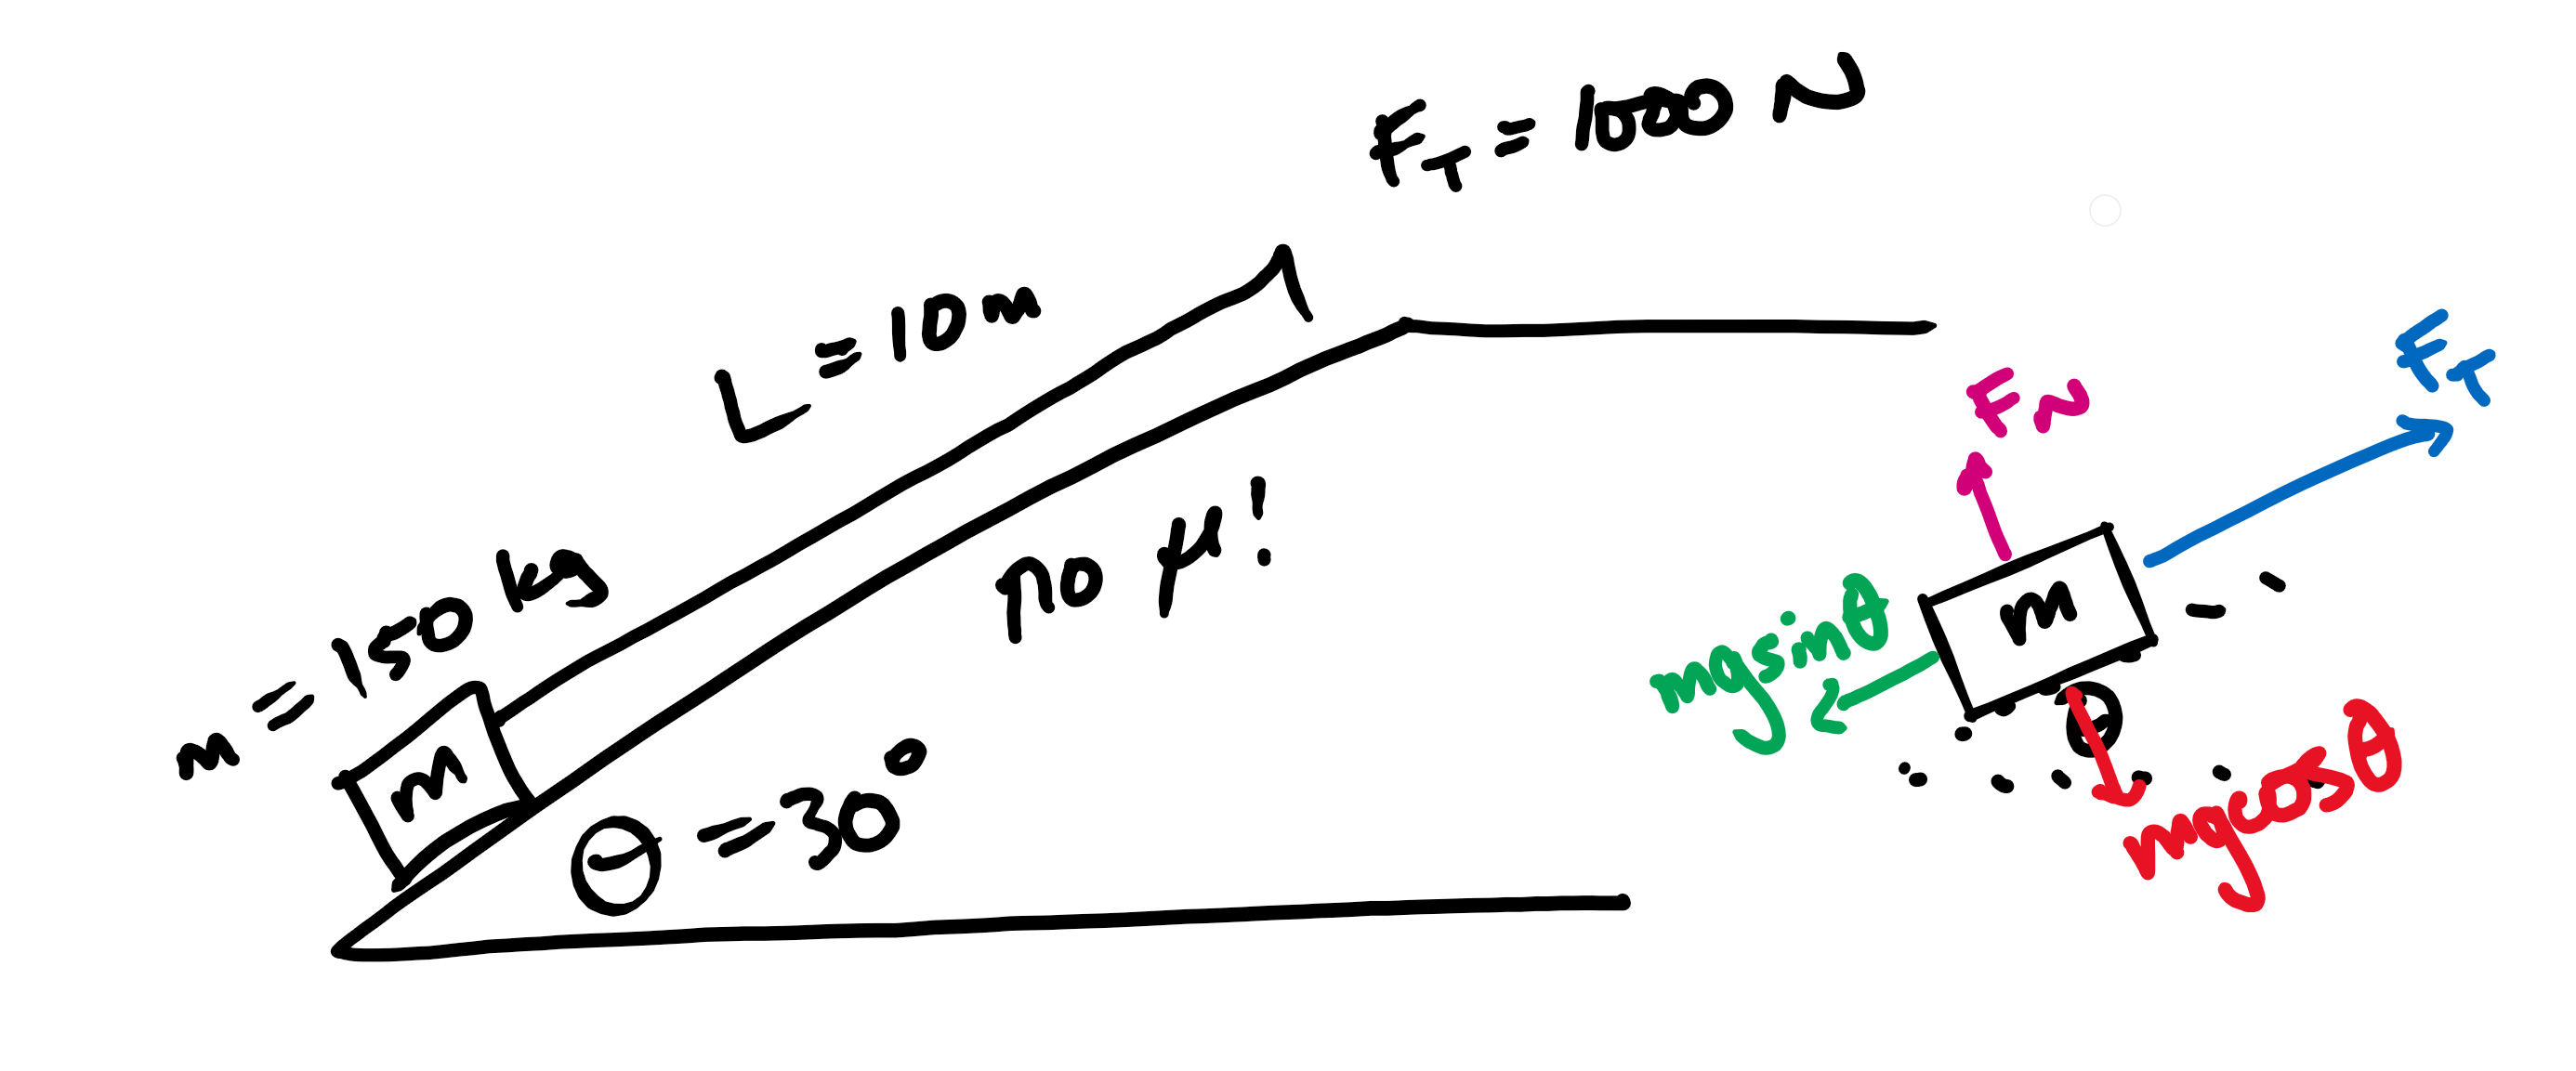
\includegraphics[width=0.5\textwidth]{chapters/ch4/images/fig4_5.PNG}
    \end{center}

    While this problem could be solved using kinematics and Newton's second law, we can also use the Work-Energy theorem. 

    $$
    \begin{aligned}
        W_{in} &= \Delta KE + \Delta PE\\
        F_T \cdot L &= \frac{1}{2}m(v_f - v_i)^2 + mg(h_f - h_i)\\
        F_T \cdot L &= \frac{1}{2}mv_f^2 + mgh_f\\
        v_f &= \sqrt{\frac{2(F_TL - mgh_f)}{m}}\\
        v_f &= \sqrt{\frac{2(F_TL - mg(L\sin\theta))}{m}}
    \end{aligned}
    $$
\end{problem}

\begin{problem}
    A skiier starts at the top of a mountain and is attached a spring at the bottom of the cliff. The skiier will also experience friction for 15m at the bottom of the slope right before the spring. How far was the spring compressed when the skiier reaches the bottom of the slope?

    \begin{center}
        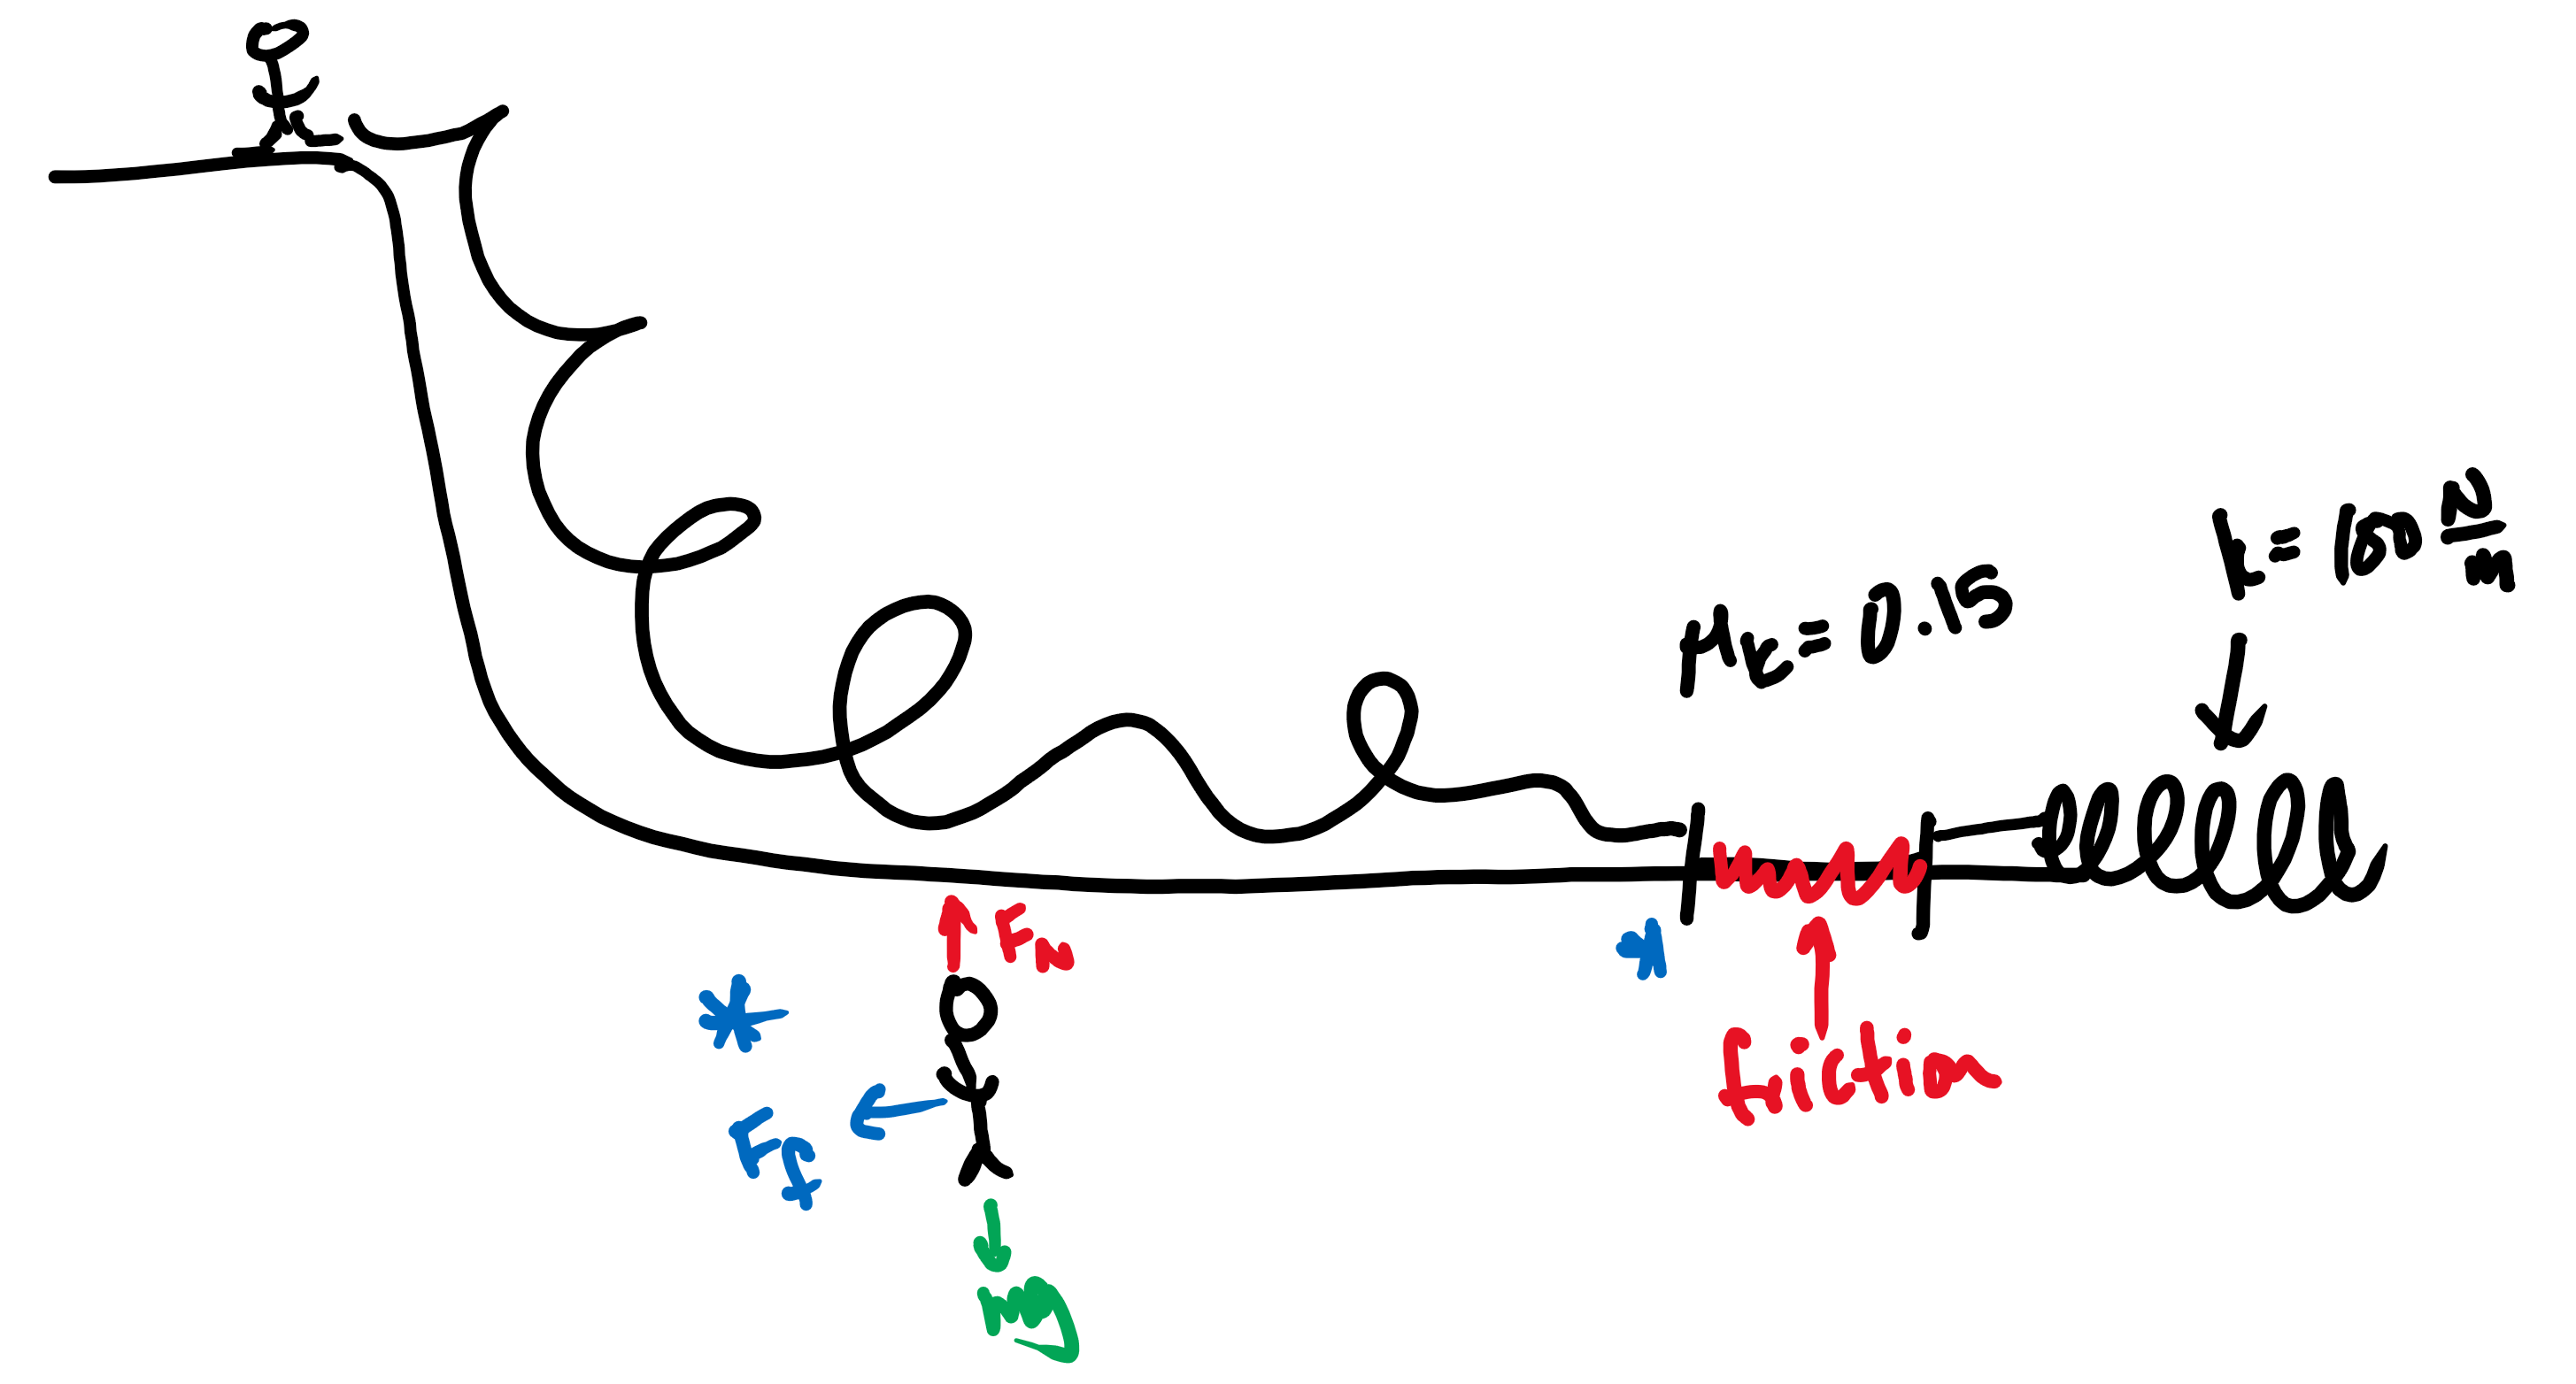
\includegraphics[width=0.5\textwidth]{chapters/ch4/images/fig4_6.PNG}
    \end{center}

    $$
    \begin{aligned}
        W_{in} = 0 &= \Delta PE + \Delta E_s + \Delta E_{T}\\
        0 &= mg(h_f-h_i) + \frac{1}{2}k(x_f-x_i)^2 + \mu_kmgD\\
        0 &= -mgh_i + \frac{1}{2}kx_f^2 + \mu_kmgD\\
        x_f &= \sqrt{\frac{(mgh_i-\mu_kmgD)^2}{k}}\\
        x_f &= \sqrt{\frac{((70\kg)(9.81\frac{\m}{\s^2})(50\m)-(0.15)(70\kg)(9.81\frac{\m}{\s^2})(15\m))^2}{150 \frac{\N}{\m}}}\\
    \end{aligned}
    $$
\end{problem}


\begin{problem}
    A stunt artist was launched out of a cannon on a 20m pedestal. He will land in a bucket attached to a pulley. The pulley also has a 50kg mass attached to it, and the bucket is 10m above the ground. Assume the bucket has no mass and the pulley exerts no friction on the string wrapped around the pulley. What is the speed of the stunt artist right when he lands in the bucket? 
    
    \begin{center}
        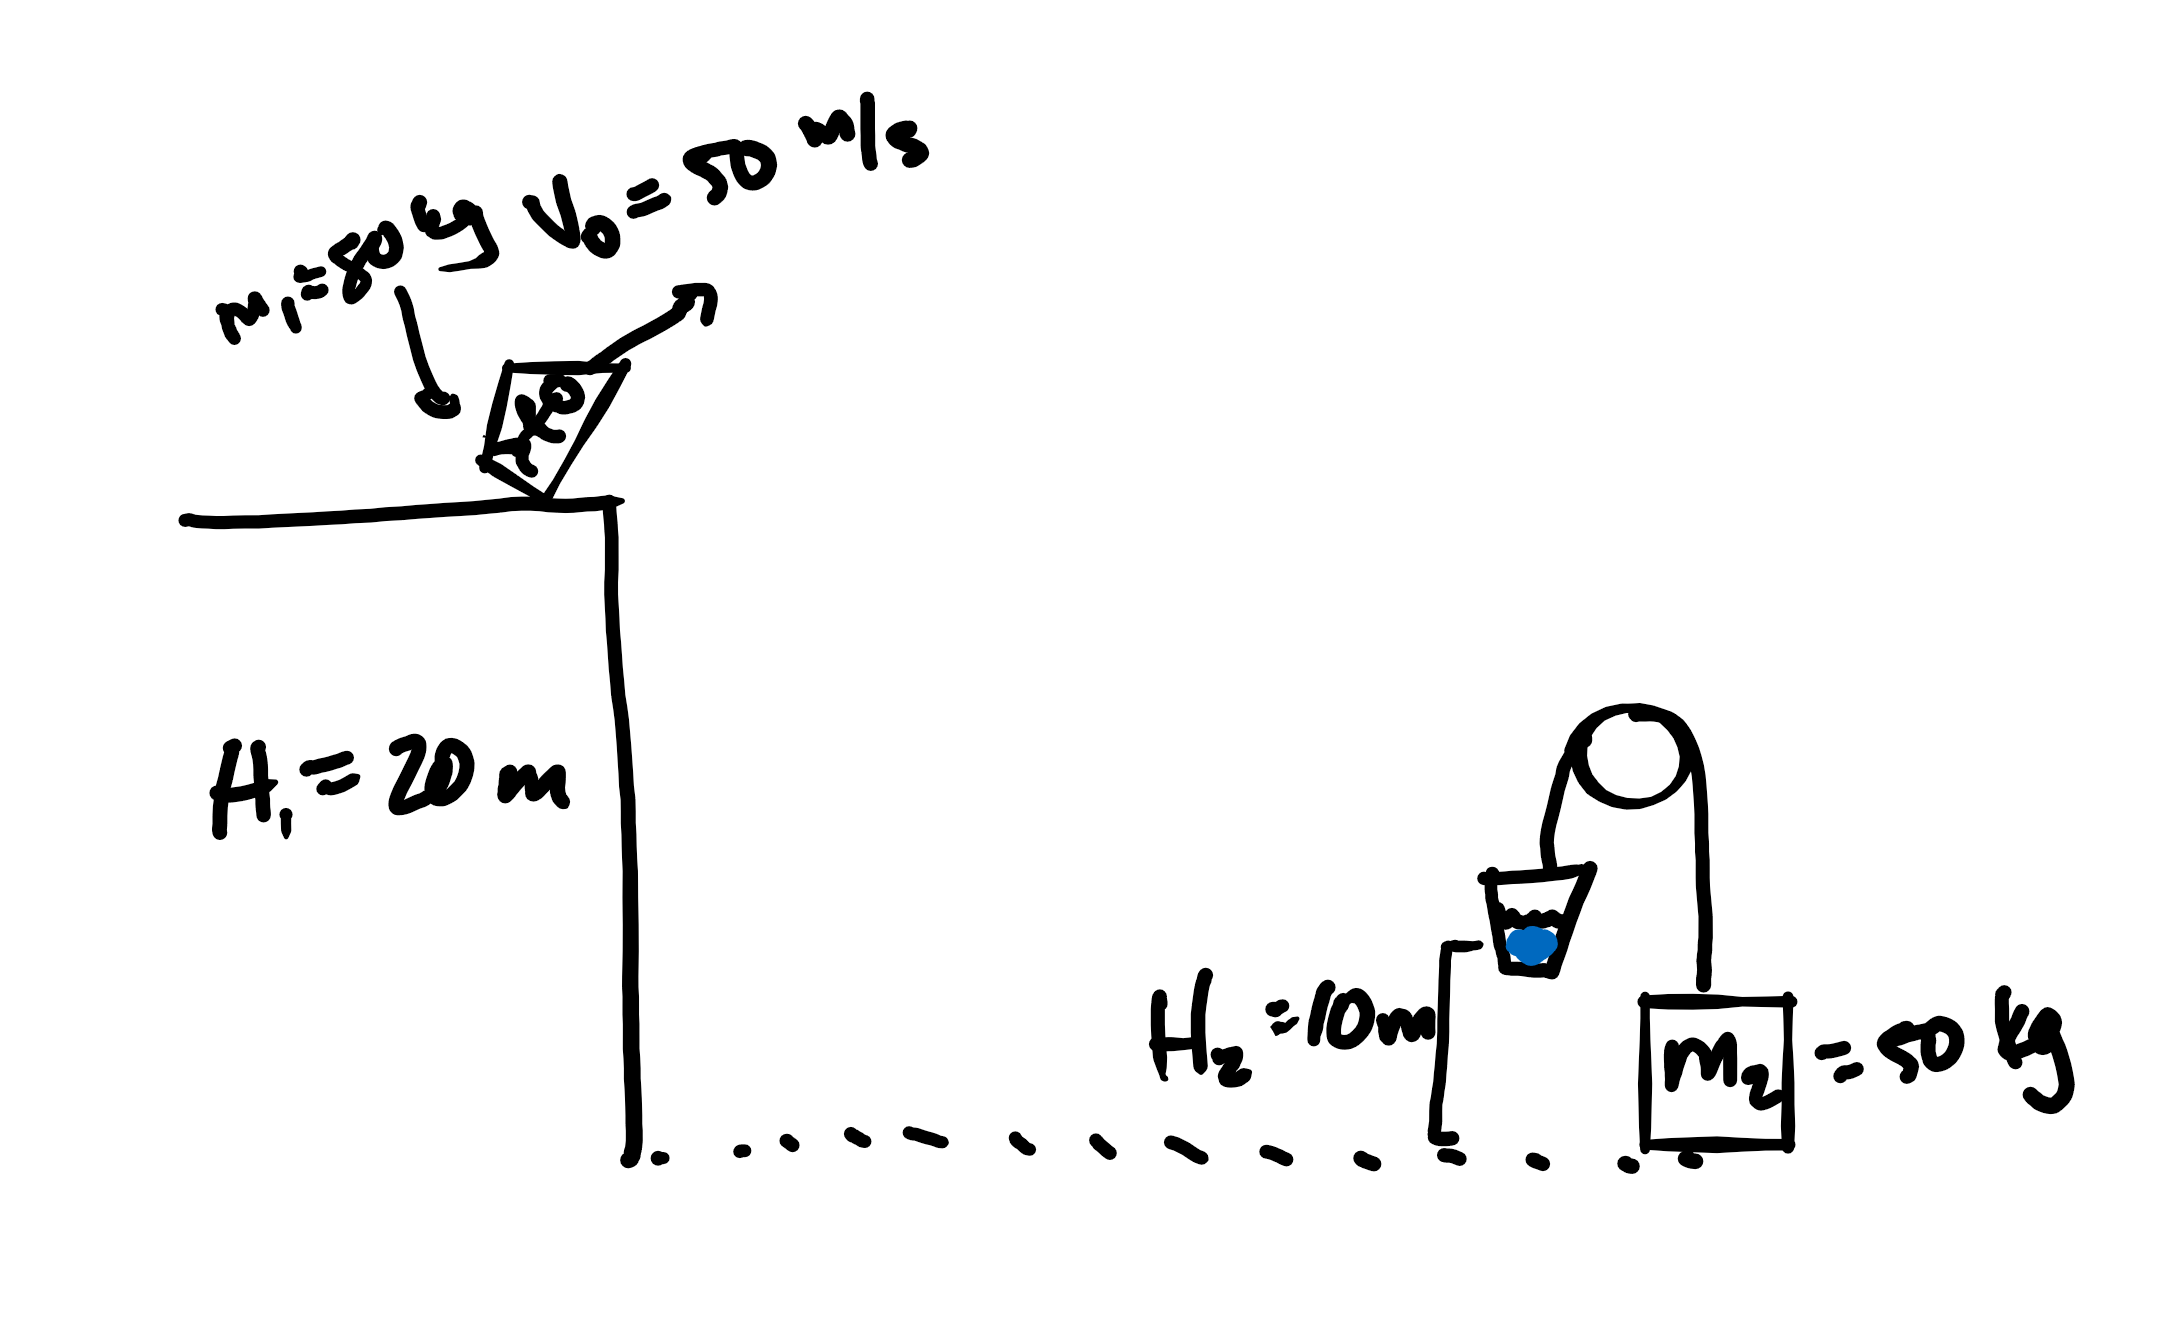
\includegraphics[width=0.5\textwidth]{chapters/ch4/images/fig4_7.PNG}
    \end{center}

    $$
    \begin{aligned}
        W = 0 &= \Delta KE_1 + \Delta PE_1 + \Delta KE_2 + \Delta PE_2\\
        0 &= \frac{1}{2}m(v_{f1}-v_{i1})^2 + \frac{1}{2}m_2(v_{f2}-v_{i2})^2 + m_1g(H_{f1} - H_{i1}) + m_2g(H_{f2} - H_{i2})\\
    \end{aligned}
    $$

    ANSWER: $41.3 \frac{\m}{\s}$
\end{problem}


\section{Work and Calculus}

\begin{itemize}
    \item Sometimes, the force being applied to an object over a given distance is variable
    \item If you are given an equation for what the force is (dependent on distance), then $W = \int_{x_i}^{x_f} F(x) dx$
\end{itemize}


\begin{problem}
    If the force applied to an object (as a function of distance) is $F(x) = 5 - 2x$, what is the work done on the object if the object moves 3 \m?

    $$
    \begin{aligned}
        W &= \int_{x_i}^{x_f} F(x) \: dx\\
        W &= \int_{0}^{3} 5-2x \: dx\\
        W &= (5-2(3))-(5-2(0)) = -1-5
        W &= -6 \J
    \end{aligned}
    $$
\end{problem}


\section{Power}

\begin{definition}[Power]{def4.5:label}
    \textbf{Power:} How much energy is expended over a given time interval.

    $$
    P = \frac{\Delta E}{\Delta t} = \frac{W}{t}
    $$

    \textbf{SI Units:} Watts (W)
\end{definition}


\begin{problem}
    A block of mass 1000 kg is attached to a pulley at the top of a building. The pulley is attached to a motor that uses 200 kW. What is the final velocity of the block the moment it reaches the top of the building?

    \begin{center}
        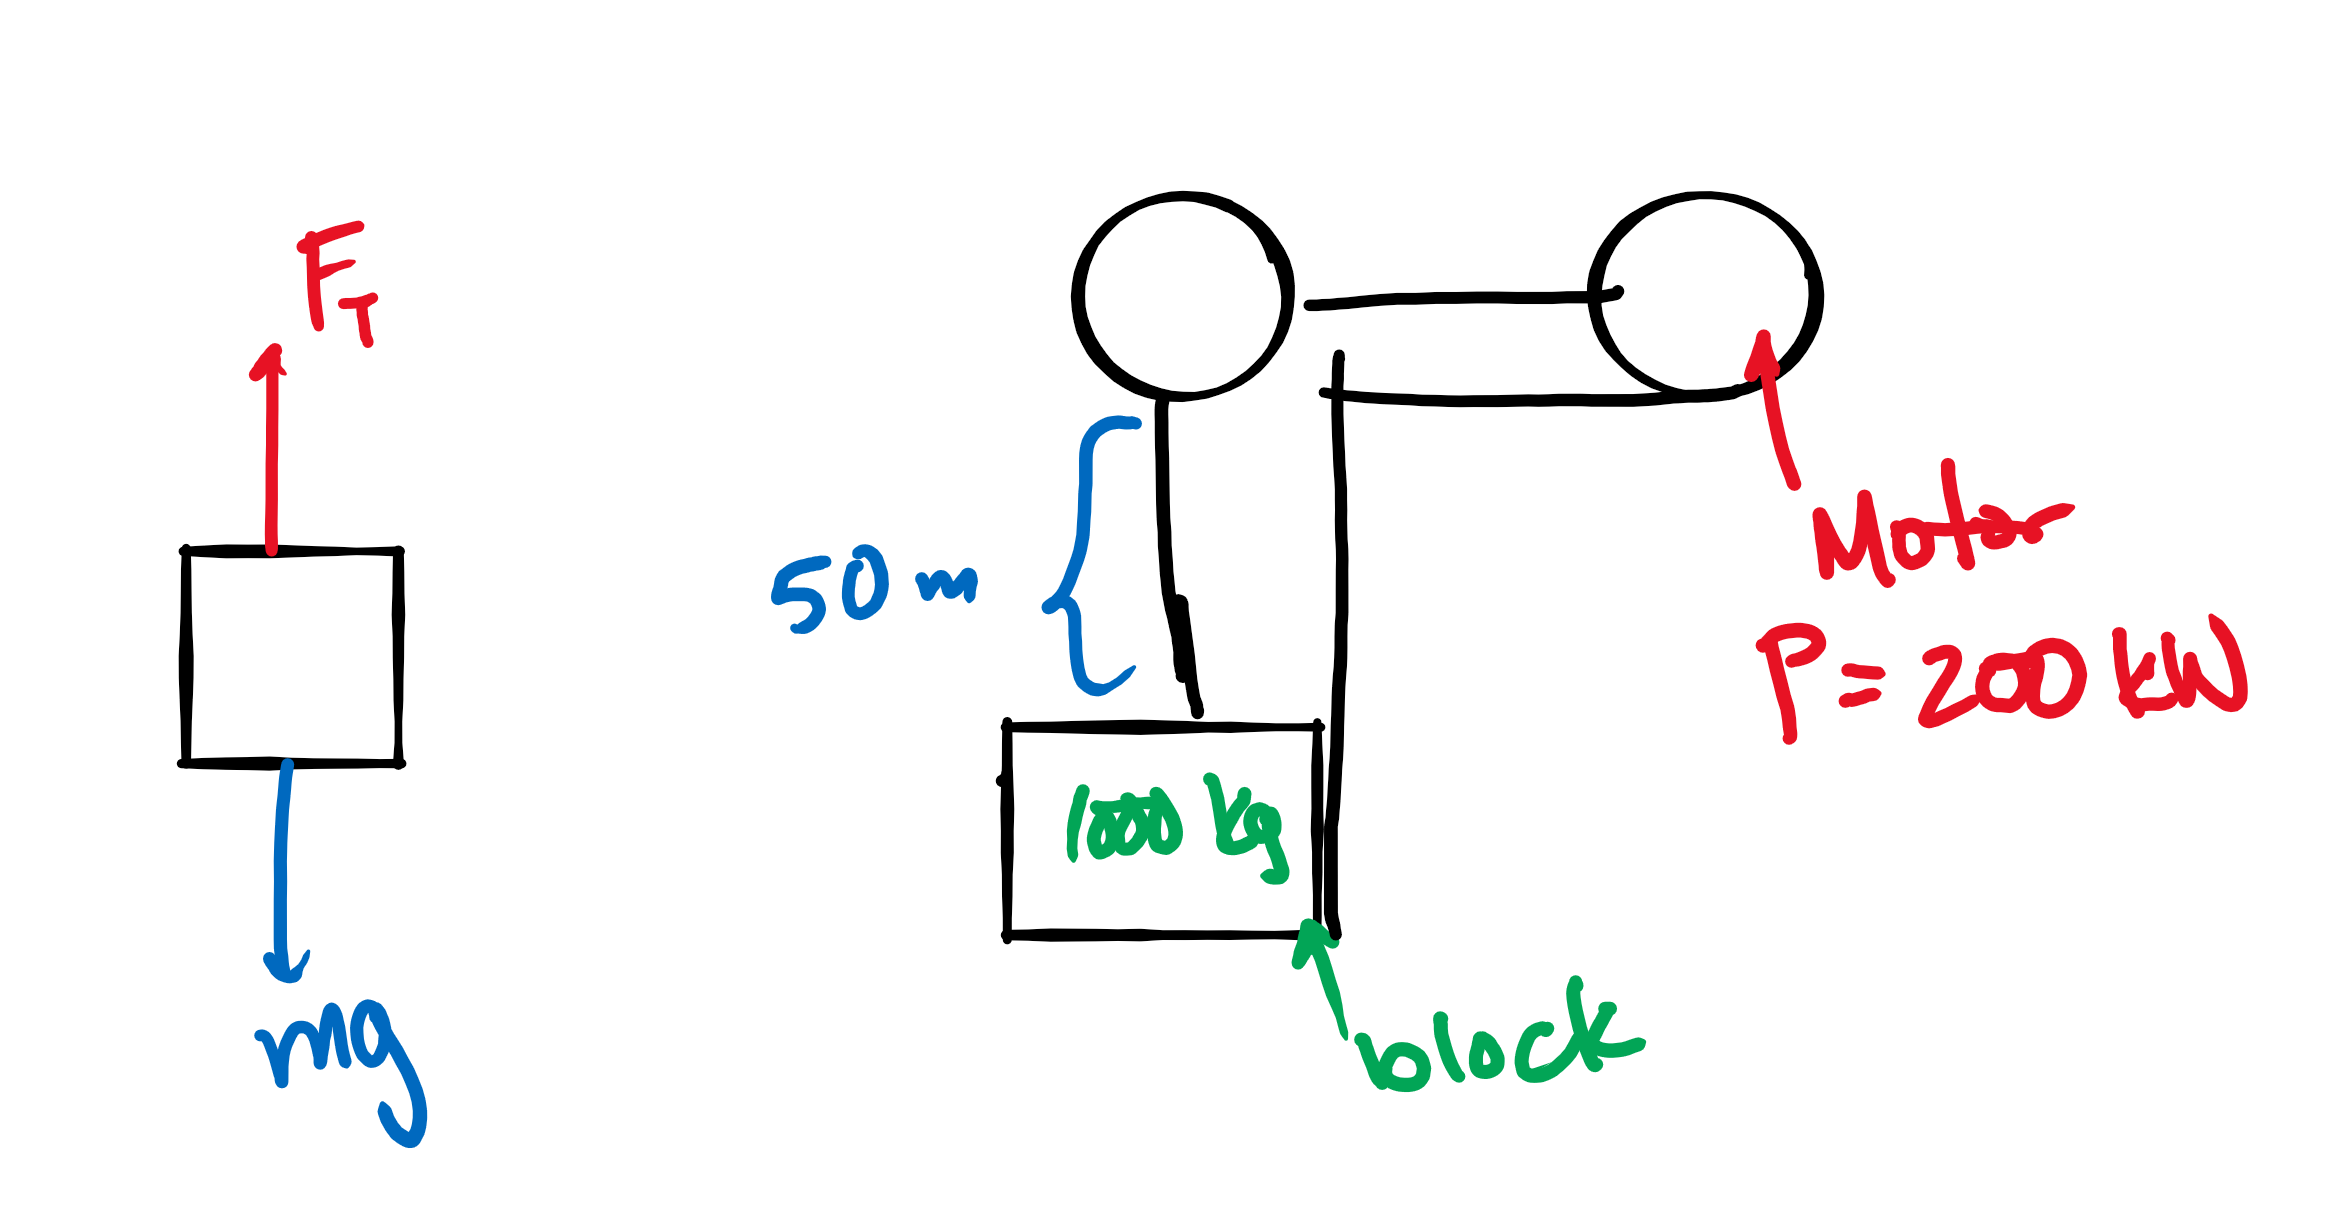
\includegraphics[width=0.5\textwidth]{chapters/ch4/images/fig4_8}
    \end{center}

    $$
    \begin{aligned}
        P &= \frac{\Delta E}{\Delta t}\\
        P &= \frac{\Delta KE + \Delta PE}{\Delta t}\\
        P &= \frac{\frac{1}{2}mv^2+mgh}{\Delta t}\\
        v_f &= \sqrt{\frac{2(-mgh+\Delta T P)}{m}}
    \end{aligned}
    $$
\end{problem}


\begin{problem}
    A truck drives up a ramp with an angle of inclination of $15^\circ$. If the truck drives 200 meters in 20 seconds, what is the power of the truck (in kW) after the truck has moved 200 meters? Assume that 10\% of the total energy is lost to the environment.

    $$
    \begin{aligned}
        P &= \frac{\Delta E}{t}\\
        P &= \frac{\Delta KE + \Delta PE}{t}+ 10\%\text{ energy}\\
        P &= \frac{\frac{1}{2}mv^2 + mgh}{t} + 10\%\text{ energy}\\
        P &= \left[\frac{\frac{1}{2}m\left(\frac{\Delta x}{t}\right)^2 + mgL\sin\theta}{t}\right]\frac{1}{0.9}\\
        P &= 98.3 \text{ kW}
    \end{aligned}
    $$
\end{problem}


\chapter{Counting}
\section{Rotational Kinematics}

\begin{itemize}
    \item While objects can move in a straight line, objects can ALSO move in a circle
    \begin{itemize}
        \item Either an object is orbiting some point or something spins around some center
    \end{itemize}
    
    \item Instead of having position, velocity, and acceleration, we will have \textit{new} terms for moving in a circle instead
    \begin{itemize}
        \item \textbf{Angular position ($\theta$):} How much the object has rotated around the positive $x$-axis
        \item \textbf{Angular velocity ($\omega$):} How fast an object is going in a given direction at any point in the circle
        \begin{itemize}
            \item $\frac{d\theta}{dt} = \omega(t)$
            \item $\theta(t) = \int \omega \: dt$
        \end{itemize}
        \item \textbf{Angular acceleration ($\alpha$):} How fast an object changes it's velocity at any point in the circle of motion
        \begin{itemize}
            \item $\frac{d\omega}{dt} = \alpha(t)$
            \item $\omega(t) = \int \alpha \: dt$
        \end{itemize}
    \end{itemize}

    \item the kinematics equations from translational (standard) motion are the EXACT SAME equations in rotational kinematics, but we simply use the rotational kinematics variables instead of the translational kinematics variables
    
    \newpage
    \begin{definition}[Rotational Kinematics Equations]{def5.1.1:label}
        To calculate different values of 

        \[
        \begin{aligned}
            \omega_f &= \omega_i + \alpha t\\
            \Delta\theta &= \omega_it + \frac{1}{2}\alpha t^2\\
            \omega_f^2 &= \omega_i^2 + 2\alpha\Delta\theta
        \end{aligned}    
        \]
    \end{definition}

    \item it is important to note that values are \textbf{positive} if things move \textit{in the counterclockwise direction} and values are \textbf{negative} if things move \textit{in the clockwise direction}
    \item If you know the distance between the object moving in rotation and the center of rotation (in other words: the radius of the circle of rotation), then you can relate the rotational kinematics values with the translational kinematics values
    
    \begin{definition}[Rotational Kinematics $\leftrightarrow$ Translational Kinematics]{def5.1.2:label}
        \[
        S = \Delta\theta R    
        \]

        Where $S$ is the arc that the object travels around through a given angle $\theta$ and $R$ is the radius (the distance between the object and the center of rotation).

        \[
        v = \omega R    
        \]

        Where $R$ is the radius (the distance between the object and the center of rotation).

        \[
        a_{tangential} = \alpha R    
        \]

        Where $R$ is the radius (the distance between the object and the center of rotation). Note that this is the acceleration that is PENPENDICULAR to the acceleration that points towards the center of the circle.

        \[
        a_{centripetal} = \frac{v^2}{R} = \frac{\omega^2 R^2}{R} = \omega^2 R    
        \]

        Where $R$ is the radius (the distance between the object and the center of rotation). Note that this is the acceleration that points towards the CENTER of the circle. 
    \end{definition}
\end{itemize}


\begin{problem}
    A grinder rotates at 850RPM. Once the grinder turns off, it stops 3 minutes later. What is the angular acceleration and what is the final anglular position of the grinder?\\

    First, convert RPM to radians/second:

    \[
    850 \frac{\text{rev}}{\text{min}}\cdot\frac{2\pi \text{ radians}}{1 \text{ rev}}\cdot\frac{1 \text{ minute}}{60 \text{ seconds}} = 28.\bar{3} \frac{\text{radians}}{\s}   
    \]

    Now find angular acceleration:
    \[
    \alpha = \frac{\Delta \omega}{t} = \frac{\omega_f - \omega_i}{t} = \frac{- 28.3 \frac{\rad}{\s}}{60 \s} = -0.49 \frac{\rad}{\s^2}   
    \]

    Now find the final angular position:
    \[
    \begin{aligned}
        \omega_f^2 &= \omega_i^2 + 2\alpha\Delta\theta\\
        \theta_f &= \frac{\omega_f^2 - \omega_i^2}{2\alpha} + \theta_i\\
        \theta_f &= \frac{-(28.\bar{3} \frac{\rad}{\s})^2}{2(-0.49 \frac{\rad}{\s^2})}\\
        \theta_f &= 817.235 \rad
    \end{aligned}    
    \]
\end{problem}


\begin{problem}
    An object rotates and has a function that defines the angluar acceleration to be $\alpha(t) = 5t^3 - 4t$. You know that the initial rotational velocity is 5 $\frac{\rad}{\s}$ and the initial angular position is 2 radians. 

    \[
    \begin{aligned}
        \omega(t) &= \int_0^t \alpha(t)\:dt\\
        \omega(t) &= \int_0^t 5t^3 - 4t \: dt\\
        \omega(t) &= \frac{5}{4}t^4 - 2t^2 + 2
    \end{aligned}    
    \]
\end{problem}


\section{Moment of Inertia}

\textbf{Intertia} is the distribution of mass around the object's center of mass. This term allows us to differentiate between a disk and a chair that are both 5kg because up to this point we have tretaed those two objects as the same object. 


\section{Force, Energy, and Momentum in Rotation}

\begin{itemize}
    \item In the \textbf{linear world}, $KE = \frac{1}{2}mv^2$, but in the \textbf{rotational world} $KE = \frac{1}{2}I\omega^2$
    \item  In the \textbf{linear world}, $F = ma$, but in the \textbf{rotational world} $\tau = I\alpha$
    \begin{itemize}
        \item It shuold be noted that the above is Newton's Second Law just applied to rotation. Individual torques are $\tau_A = F_Ar\sin\theta$ where $r$ is the distance between the center of rotation and the point where the force is applied.
    \end{itemize}
    \item In the \textbf{linear world}, $W = F \cdot d$, but in the \textbf{rotational world} $W = \tau \cdot \theta$
    \item In the \textbf{linear world}, $P = Fv$, but in the \textbf{rotational world} $P = \tau\omega$
    \item In the \textbf{linear world}, $p = mv$, but in the \textbf{rotational world} $L = I\omega$
\end{itemize}

\begin{problem}
    \begin{center}
        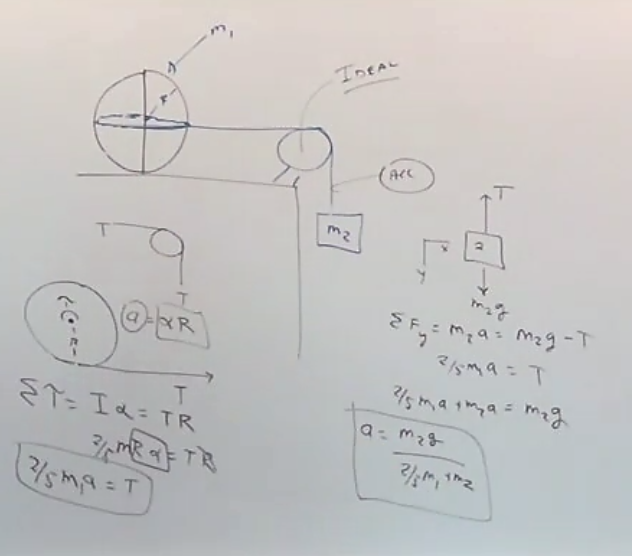
\includegraphics[width=0.75\textwidth]{chapters/ch5/images/fig5_1.PNG}
    \end{center}
\end{problem}

\begin{problem}
    \begin{center}
        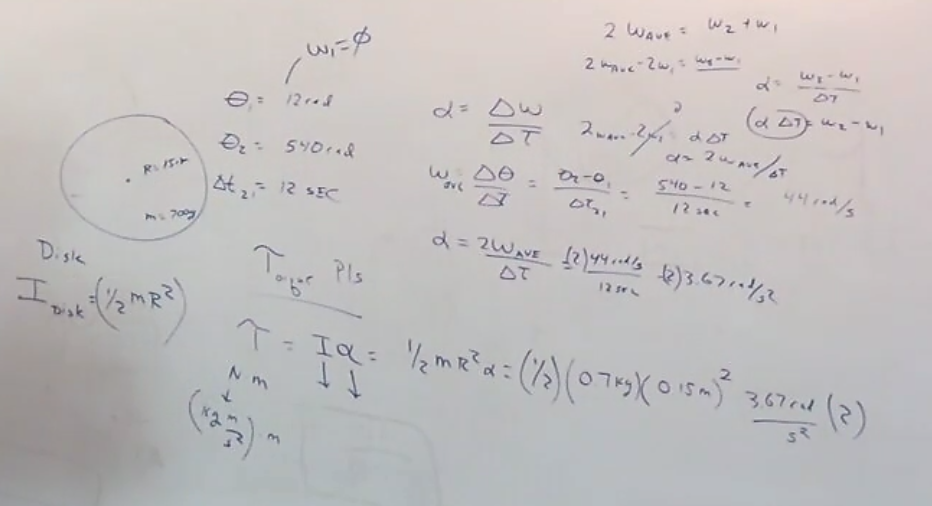
\includegraphics[width=0.75\textwidth]{chapters/ch5/images/fig5_2.PNG}
    \end{center}
\end{problem}


\section{Smooth Rolling Motion}

\[
\begin{aligned}
    \sum F_x  &= ma_{COM} = F_f\\
    \sum \tau_{NET} &= I\alpha = \tau_{APP} - \tau_f = \tau_{APP} - F_fR
\end{aligned}    
\]



\section{Newton's Second Law for Rotation}

\[
\begin{aligned}
    \tau &= I\alpha\\
    F_fR &= I\alpha\\
\end{aligned}    
\]


\section{Angular Momentum and Impulse}

\begin{itemize}
    \item We've been used to \textit{linear momentum} but there is also \textbf{angular momentum} that functions under the same properties
    
    \begin{definition}[Angular Momentum]{def5.6.1:label}
        \[
        L = I\omega     
        \]

        In every case in this class, \textbf{angular momentum will always be conserved}
    \end{definition}

    \item Angular momentum is the reason that an ice skater changes their speed
    \begin{itemize}
        \item When the skater holds out their arms, then the 
    \end{itemize}
\end{itemize}

\begin{problem}[Merry Go Round]
    \[
    \begin{aligned}
        L_i &= L_f\\
        I_m\omega_i &= I_m\omega_f + I_\parallel\omega_f\\
        \omega_f &= \frac{I_m\omega_i}{I_m + I_\parallel}
    \end{aligned}    
    \]
\end{problem}


\begin{problem}[Merry Go Round with Dog]
    \[
    \begin{aligned}
        L_i &= L_f\\
        I_m\omega_i + I_D\omega_i &= I_m\omega_f + I_D(\omega_f - \omega_D)
    \end{aligned}    
    \]
\end{problem}

\begin{itemize}
    \item Additionally, we can get an angular impulse similarly to how we get a linear impulse
    
    \begin{definition}[Angular Impulse]{def5.6.2:label}
        \[
        J_\angle = \tau_{AVG}\Delta T = I \Delta \omega      
        \]
    \end{definition}
\end{itemize}


\begin{problem}[Grindstone Problem]
    \[
    \begin{aligned}
        L_i &= L_f\\
        I_1\omega_i &= I_1\omega_f + I_2\omega_f\\
        I_1\omega_i &= \omega_f(I_1 + I_2)\\
        \omega_f &= \frac{I_1}{I_1+I_2}\omega_i\\
        \omega_f &= \frac{0.5M_1R_1^2}{0.5M_1R_1^2+0.5M_2R_2^2}\omega_i\\
    \end{aligned}    
    \]
\end{problem}


\chapter{Advanced Counting}



\chapter{Relations}
\section{Recursive Relations and Recursive Definitions}

\begin{problem}
    Find the first four terms of the sequence if:

    \begin{itemize}
        \item $f(n+1) = 3f(n);\:\:\:f(0)=2$
        \begin{itemize}
            \item $f(1)=3f(0)=3(2)=6$
            \item $f(2)=3f(1)=3(6)=18$
            \item $f(3)=3f(2)=3(18)=54$
            \item $f(4) = 3f(3)= 3(54) = 162$
        \end{itemize}
    \end{itemize}
\end{problem}

\begin{problem}
    A ternary is a string consisting of 0s, 1s, and 2s.

    \begin{itemize}
        \item Find a recurrence relation for the number of ternary strings of length $n$ that contain a pair of consecutive 2s.
        \begin{itemize}
            \item $a_n = 2a_{n-1} + 2a_{n-2} + 3^{n-2}$
        \end{itemize}

        \item What are the initial condition(s)?
        \begin{itemize}
            \item $a_2 = 2$
            \begin{itemize}
                \item 22
            \end{itemize}
            \item $a_3 = 5$
            \begin{itemize}
                \item 220
                \item 221
                \item 222
                \item 022
                \item 122
            \end{itemize}
            \item $a_4 = 2a_3 + 2a_2 + 3^2 = 21$ 
        \end{itemize}

        \item Determine the number of ternary strings of length 5 that contain a pair of consecutive 2s.
        \begin{itemize}
            \item $a_5 = 2a_4 + 2a_3 + 3^3 = 2(21)+2(5)+3^3 = 79$
        \end{itemize}
    \end{itemize}
\end{problem}



\section{Solving Linear Recurrence Relations}

\begin{itemize}
    \item a sequence $\{a_n\}$ is a \textbf{solution} to a recurrence relation if its terms satisfy the recurrence relation
\end{itemize}


\begin{problem}
    Which of the following sequences are solutions of the recurrence relation $a_n = 8a_{n-1} - 16a_{n-2}$?

    \begin{itemize}
        \item $a_n = 0$ $\implies$ [ADD WORK LATER] 
        \item $a_n = 2^n$ \textbf{is NOT a solution}
        \[
        \begin{aligned}
            &8\cdot 2^{n-1}-16\cdot 2^{n-2}\\
            &2^3\cdot 2^{n-1}-2^4\cdot 2^{n-2}\\
            &2^{n+2} - 2^{n+2} = 0
        \end{aligned}    
        \]
        \item $a_n = 3n4^n$ \textbf{IS a solution}
        \[
        \begin{aligned}
            &8\cdot 3(n-1)\cdot 4^{n-1} - 16 \cdot 3(n-2) \cdot 4^{n-2}\\
            &2\cdot 4\cdot 3(n-1)4^{n-1} - 4\cdot 4 \cdot 3 (n-2) 4^{n-2}\\
            &6(n-1)4^n - 3(n-2)4^n\\
            &4^n(6n-6-3n+6)\\
            &3n4^n
        \end{aligned}    
        \]
    \end{itemize}
\end{problem}

\subsection{Solving Recurrence Relations}


If the recurrence relation only depends on \textbf{one term}, use the following process:
\begin{itemize}
    \item To solve a recurrence relation $a_n=ca_{n-1}$, look at the root of the equation $r-c=0$
    \item the root is $r_1 = c$
    \item genereal form of the solution then is $a_n=\alpha (r_1)^n$ such that $n \ge 0$
    \item Use the initial condition to solve for $\alpha$
\end{itemize}

If the recurrence relation depends on \textbf{two terms}, use the following process:

\begin{itemize}
    \item To solve a recurrence relation $a_n=c_1a_{n-1} + c_2a_{n-2}$, look at the root of the equation $r^2-c_1r-c_2=0$
    \item the roots can be found using the quadratic fomula or by factoring
    \item genereal form of the solution then is $a_n=\alpha (r_1)^n + \beta (r_2)^n$ such that $n \ge 0$
    \item Use the initial conditions to solve for $\alpha$ and $\beta$
\end{itemize}


\begin{problem}
    Solve $a_n = 5a_{n-1}\:\:\:(n\ge 1),\:\: a_0 = -2$.
\end{problem}

\begin{problem}
    Solve $a_n = a_{n-1}+6a_{n-2}\:\:\:(n\ge 2),\:\: a_0 = 3 \:\&\: a_1 = 6$.
\end{problem}


\chapter{Graphs}
\section{Graphs and Terminology}

\begin{definition}
    A \textbf{graph} $G=(V,E)$ consists of a nonempty set of vertices and a set $E$ of edges. Each edge has either one or two vertices associated with it, called its \textit{endpoints}. A \textbf{loop} is an edge between a vertex and itself. A \textbf{multiple edge} is one in which the same pair of vertices is assigned to the more than one edge.  
\end{definition}



\chapter{Trees}

\end{document}
